\documentclass[../main.tex]{subfiles}
\addbibresource{../bibfile.bib}

\begin{document}

\chapter{Analisi implementate}
In questo capitolo, verranno descritte nel dettaglio le tecniche di ricerca automatica delle vulnerabilità rese disponibili dalla piattaforma.
In particolare, verranno illustrate quali metodologie di analisi ogni tecnica utilizza e come esse concorrono al rilevamento
di particolari classi di vulnerabilità.
\section{VulnDetect}
Le tecniche che si basano sull'esecuzione simbolica devono tenere conto del problema noto con il nome di \textit{path explosion}: l'incremento delle
dimensioni di un programma porta ad un aumento esponenziale dei cammini praticabili presenti sul suo CFG, i quali possono crescere fino a diventare
potenzialmente infiniti se il programma contiene cicli non vincolati da una condizione di terminazione \cite{SE_Path_explosion}. 
Per evitare questo problema, l'esecutore simbolico può essere guidato in modo tale che esplori solamente una parte del CFG del programma, in modo tale da evitare che esso
esplori cammini potenzialmente inutili alla ricerca di vulnerabilità. \textbf{VulnDetect} \cite{VulnDetect} è una tecnica di ricerca basata su esecuzione simbolica per la ricerca
di vulnerabilità di tipo \textbf{stack-based buffer-overflow}. L'implementazione di VulnDetect si basa sulle funzionalità offerte dalla piattaforma \textit{angr}.
Per evitare il problema della \textit{path explosion}, VulnDetect utilizza un insieme di metodologie di analisi statica per guidare
l'esecutore simbolico ad analizzare solo i cammini potenzialmente vulnerabili del programma.
\subsection{Buffer overflow e Stack-Based Buffer Overflow}
Una delle classi di vulnerabilità software più diffuse nel panorama software moderno è quella che prende il nome di \textbf{buffer overflow} (CWE-120).
Questo tipo di vulnerabilità si presenta quando non avviene nessun controllo sulla lunghezza massima dei dati che devono essere salvati all'interno
di un buffer allocato in memoria. Il dato, quindi, può potenzialmente andare a sovrascrivere i dati posti in sezioni di memoria adiacenti all'area di allocazione
del buffer, potenzialmente quindi andando a sovrascrivere dati fondamentali per la corretta esecuzione del programma. 
Questa problematica è particolarmente rilevante nei linguaggi non \textit{memory safe}, dove il compito di gestione della memoria del programma è affidato
al programmatore. Quando il buffer-overflow può avvenire su un buffer allocato nello stack del programma, la vulnerabilità prende il nome di \textbf{stack-based buffer overflow} (CWE-121).
La presenza di questo tipo di vulnerabilità può portare a conseguenze catastrofiche: un attaccante, per esempio, potrebbe sovrascrivere l'indirizzo di ritorno della funzione in cui viene dichiarato il buffer, 
potenzialmente portando il programma ad eseguire codice malevolo presente nell'input (shellcode).
\subsection{Strategia di analisi}
VulnDetect struttura la strategia di analisi in due fasi distinte \cite{VulnDetect}:
\begin{enumerate}
    \item \textbf{Analisi statica}: Le vulnerabilità di tipo \textit{buffer overflow} sono principalmente causate dall'utilizzo improprio di funzioni pericolose (in C, per esempio \textit{gets, scanf,}...) e dalla mancanza di controlli
    sulla lunghezza dell'input dell'utente. Per migliorare l'efficienza dell'esecuzione simbolica, VulnDetect applica una sequenza di tecniche di analisi statica sul programma:
    \begin{enumerate}
        \item \textbf{Identificazione di operazione sensibili}: Innanzitutto, viene caricato il programma tramite la classe \textit{Project} di angr.
        Successivamente, si procede al recupero degli indirizzi delle funzioni di libreria potenzialmente pericolose, accedendo alle informazioni contenute nella \textit{Procedure Linkage Table} (PLT).
        Per determinare quali funzioni recuperare dalla PLT, il programma di analisi mantiene al suo interno una \textbf{lista di nomi di funzioni potenzialmente pericolose}.
        Viene infine recuperato, sempre tramite angr, il CFG del programma, il quale viene attraversato in modo tale da individuare \textbf{gli indirizzi nel programma in cui avvengono chiamate a funzioni pericolose}.
        \item \textbf{Program slicing}: Per prima cosa, viene creato il Data Dependency Graph del programma. Dopodiché, viene effettuato \textit{program slicing} per ogni indirizzo di chiamata a funzione pericolosa individuato nel passo precedente, in modo tale
        da estrarre i segmenti di codice correlati ad ogni chiamata. Chiameremo questi segmenti \textit{hotspot code segments}.
    \end{enumerate}
    \item \textbf{Vulnerability detection}: La ricerca di vulnerabilità viene effettuata eseguendo simbolicamente il programma, simulando l'input dell'utente con un \textbf{input simbolico}. Per evitare \textit{path explosion}, l'esecutore simbolico viene guidato durante il processo di esecuzione usando gli \textit{hotspot code segments} ottenuti
    durante la fase di analisi statica. Così facendo, l'esecuzione simbolica esplorerà solamente i cammini legati alla ricerca della vulnerabilità, invece di tutti i cammini praticabili del CFG. Quando l'esecuzione arriva ad un punto del programma dove avviene una chiamata ad una funzione pericolosa, è necessario 
    continuare da quel punto l'esecuzione simbolica del programma per assicurarsi che l'operazione che svolge porti ad una vulnerabilità. In caso di presenza di buffer overflow, il registro \textit{EIP} (Extended Instruction Pointer) conterrà un valore simbolico. Questo stato non permette quindi all'esecutore di determinare quale sarà il prossimo
    stato in cui si troverà il programma e quindi l'esecuzione viene interrotta. In angr, questo tipo di stati del programma prendono il nome di \textbf{unconstrained states}. 
    Sarà quindi presente nel programma una vulnerabilità di tipo \textit{stack-based buffer overflow} se l'esecutore simbolico trova almeno uno stato \textit{unconstrained} durante l'esecuzione.
\end{enumerate}
\begin{figure}[H]
    \centering
    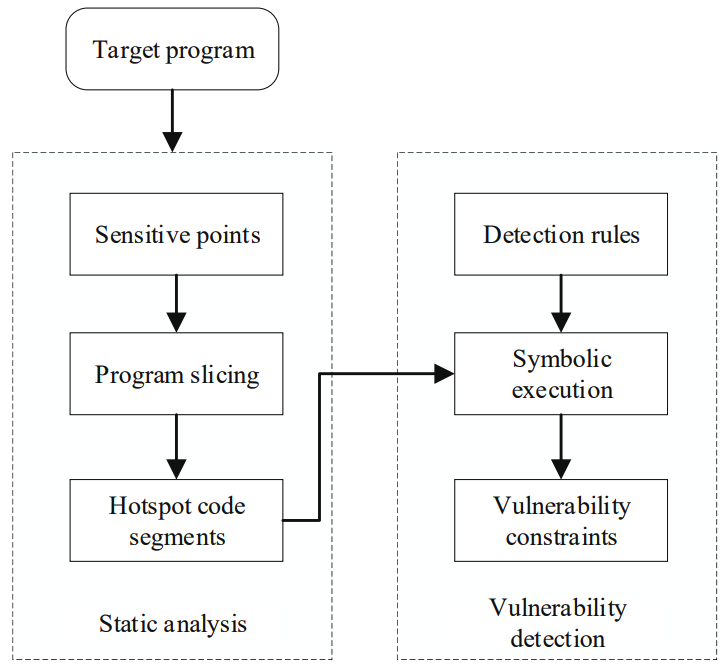
\includegraphics[width = 0.60\textwidth]{../images/VulnDetect.png}
    \caption{Processo di analisi impiegato da VulnDetect. Immagine proveniente da \cite{VulnDetect}}
\end{figure}
\section{Arbiter}
Oltre alle problematiche già discusse nel \textit{capitolo 2}, le tecniche di analisi dinamica soffrono anche di un significativo problema di \textit{scalabilità}. 
In particolare, l'esecuzione simbolica dinamica presenta una pessima scalabilità quando applicata su file binari di grandi dimensioni. 
A questo si aggiunge il problema, presente in tutte le tecniche di analisi dinamica, della bassa copertura in termini di codice analizzato.
Per essere utile all'analista, una tecnica di ricerca automatica delle vulnerabilità deve soddisfare due requisiti cruciali: la \textbf{generalità}, ossia la capacità di poter essere impiegata
su un ampio spettro di programmi, e \textbf{l'accuratezza}, la quale richiede di introdurre un numero di falsi positivi quanto più minimale possibile.
Le tecniche di \textbf{analisi ibrida} si configurano quindi come una scelta particolarmente adatta a questo scopo, in quanto combinano i punti di forza sia di analisi dinamica e statica, permettendo così di mitigarne
le problematiche. \textbf{Arbiter} \cite{Arbier} è una tecnica ibrida di ricerca automatica di vulnerabilità, progettata per individuare la presenza di diverse classi di vulnerabilità attraverso una combinazione di analisi statiche e dinamiche.
La metodologia di analisi proposta da \textit{Arbiter} permette di mitigare il numero di falsi positivi introdotti dalle tecniche di analisi statica, mantenendo al contempo una buona scalabilità al crescere delle dimensioni del programma analizzato.
L'implementazione delle tecniche di analisi usate da \textit{Arbiter} sfrutta le funzionalità messe a disposizione dal framework di analisi \textit{angr}.
\newpage
\subsection{Property-Compliant Vulnerabilities}
Arbiter è capace di rilevare tutte quelle vulnerabilità che rispettano la seguente serie di proprietà \cite{Arbier}:
\begin{itemize}
    \item \textbf{(P1): Sensibilità al flusso dei dati}: Le vulnerabilità che sono sensibili al flusso dei dati nel programma (\textit{data-flow sensitive}) possono essere rilevate effettuando
    un ragionamento riguardante il flusso dei dati dalle sorgenti di input ai sink vulnerabili. È necessario notare che il numero di questo tipo di vulnerabilità è strettamente maggiore rispetto al numero di vulnerabilità
    rilevabili effettuando solamente una \textit{taint-analysis}; quest'ultime, infatti, includono solamente quelle vulnerabilità causate da una \textbf{mancata sanificazione} dell'input dell'utente.
    \item \textbf{(P2): Sorgenti e sink facilmente identificabili}: Le sorgenti di input e i loro sink devono essere facilmente identificabili, cioè devono poter essere identificati tramite l'analisi di artefatti che è possibile
    produrre in maniera computazionalmente efficiente, come per esempio, un CFG.
    \item \textbf{(P3): Aliasing determinato dal flusso di esecuzione}: Le informazioni riguardanti l'accesso alla stessa area di memoria attraverso \textit{aliasing} devono essere recuperabili semplicemente analizzando il flusso d'esecuzione del programma.
    Questa proprietà risulta vera solamente quando il programma non effettua nessuna \textbf{deferenziazione di puntatori} oppure quando la deferenziazione può essere \textbf{risolta ad un singolo oggetto} determinato interamente dal flusso di esecuzione del programma.
\end{itemize}
Chiameremo una vulnerabilità \textit{property-compliant} (PC) quando essa rispetta tutte e tre le proprietà descritte sopra. Tuttavia, è necessario notare che la condizioni sulla deferenziazione dei puntatori descritte nella proprietà \textit{P3} portano
l'analisi a barattare ad una perdita di generalità in cambio di un aumento dell'efficienza.
\subsection{Vulnerability descriptions} 
Per effettuare l'analisi per ogni classe di vulnerabilità \textit{property-compliant}, \textit{Arbiter} utilizza una descrizione, specifica per ogni vulnerabilità, delle proprietà descritte sopra chiamata \textit{Vulnerability description} (VD).
Una VD è una \textbf{rappresentazione programmatica in linguaggio python} dei vari artefatti statici e simbolici inerenti ad ogni proprietà che una vulnerabilità property-compliant deve rispettare.
Una VD contiene le seguenti funzioni:
\begin{itemize}
    \item \textbf{specify\_sources(binary)}: Questa funzione deve ritornare un dizionario contenete tutte le sorgenti di input (funzioni) potenzialmente malevole  del programma. Ad ogni chiave del dizionario può
    essere associato il valore numerico $0$, il quale indicherà ad \textit{Arbiter} di tracciare il flusso di dati generato dal valore di ritorno della funzione, oppure un valore numerico $i > 0$, il quale indicherà ad \textit{Arbiter} di
    tracciare il flusso di dati generato dal parametro $i$-esimo della funzione.
    \item \textbf{specify\_sinks(binary)}: Similmente a \textit{specify\_sources}, questa funzione deve ritornare un dizionario contenete tutti i potenziali sink (funzioni) dei flussi di dati vulnerabili. Ad ogni funzione nel dizionario è associata una lista di caratteri così strutturata:
    \begin{itemize}
        \item Se la cella $j$-esima contiene il carattere $n$, allora \textit{Arbiter} considererà i flussi di dati che arrivano ad essere utilizzati come parametro $j$-esimo della funzione.
        \item Se la cella $j$-esima contiene il carattere $c$, allora \textit{Arbiter} ignorerà i flussi di dati che arrivano ad essere utilizzati come parametro $j$-esimo della funzione
    \end{itemize}
    \item \textbf{apply\_constraints(state, sources, sink)}: Questa funzione specifica, utilizzando le funzionalità di \textit{claripy} tramite \textit{angr}, quali sono le condizioni che il flusso di dati da sorgente a sink deve rispettare
    per essere considerato vulnerabile.
\end{itemize}
Le VD attualmente presenti in \textit{Arbiter} coprono le seguenti classi di vulnerabilità:
\begin{table}[H]
\centering
\begin{tabularx}{\textwidth}{|l|X|X|X|}
\hline
CWE     & Descrizione                                        & Sorgente                        & Sink                                                                                                   \\ \hline
CWE-131 & Incorrect calculation of buffer size               & Qualsiasi operazione aritmetica & 1° argomento di malloc()                                                                               \\ \hline
CWE-134 & Controlled format string                           & Qualsiasi dato in input         & Tutte le funzioni della famiglia di printf()                                                           \\ \hline
CWE-252 & Unchecked return value                             & Valore di ritorno di setuid()   & Qualsiasi operazione che usa il dato generato dalla sorgente                                           \\ \hline
CWE-337 & Predictable seed in pseudo-random number generator & Valore di ritorno di time()     & 1° argomento di srand()                                                                                \\ \hline
\end{tabularx}
\caption{Vulnerability description attualmente disponibili in Arbiter}
\end{table}
\noindent
Inoltre, è possibile creare delle VD per le seguenti classi di vulnerabilità:
\begin{table}[H]
\centering
\begin{tabularx}{\textwidth}{|l|X|X|X|}
\hline
CWE     & Descrizione                                        & Sorgente                        & Sink                                                                                                   \\ \hline
CWE-78 & OS Command injection& 1° argomento di sprintf() & 1° argomento di system()                                                                               \\ \hline
CWE-190 & Integer overflow or Wraparound                           & Operazione aritmetica sul valore di ritorno di sizeof()         & Qualsiasi parametro di funzione di tipo size\_t                                                           \\ \hline
CWE-676 & Use of potentially dangerous function                             & Qualsiasi funzione   & 1° argomento di strcopy()                              \\ \hline
CWE-120 & Classic buffer overflow     & 2° argomento di read() & 1° argomento di memcpy()                                                                                \\ \hline
\end{tabularx}
\caption{Classi di vulnerabilità per le quali è possibile scrivere una VD}
\end{table}
\subsection{Strategia di analisi}
Supponiamo di voler analizzare il programma $P$ per controllare se esso presenta una certa vulnerabilità $V$.
Allora, \textit{Arbiter} struttura la strategia di analisi per $V$ nelle seguenti fasi:
\begin{enumerate}
    \item \textbf{Control Flow Recovery}: Viene innanzitutto effettuato il recupero del Control Flow Graph del programma tramite le funzionalità offerte da \textit{angr}.
    \item \textbf{Subject Caller Identification}: \textit{Arbiter} utilizza il CFG e le informazioni presenti nella VD di $V$ per identificare nel programma le sorgenti di input potenzialmente malevole e i loro sink. 
    \item \textbf{Data Dependency Recovery}: Viene costruito un DDG per ogni funzione che contiene almeno una sorgente o un sink descritto nella VD di $V$. 
    Se la VD di $V$ descrive sia sorgenti che sink, allora il DDG costruito per una certa funzione $f$ non conterrà alcuna informazione riguardante le funzioni che
    chiamano $f$. Altrimenti, verrà costruito un DDG per ogni funzione, sia chiamata che chiamante, che contiene almeno un sink descritto nella VD, invece di costruire in DDG che copra
    tutte le potenziali sorgenti di input. Questo meccanismo rende la generazione del DDG per il programma più scalabile, al costo, tuttavia, di una perdita di precisione; la quale verrà
    corretta durante la fase di verifica finale dei risultati.
    \item \textbf{Backward Slicing e Filtering}: L'identificazione dei flussi potenzialmente vulnerabili avviene tracciando i cammini che collegano le sorgenti ai sink sul DDG e generando i \textbf{sotto-grafi}
    corrispondenti a tali cammini. Tale processo è equivalente all'effettuare un \textit{program slicing} statico sul programma per ogni flusso di interesse.
    \item \textbf{Under Constrained Symbolic Execution (UCSE)}: I flussi di dati raccolti durante le fasi precedenti potrebbero non essere realmente vulnerabili: la path condition che caratterizza un determinato flusso di dati
    potrebbe infatti risultare \textbf{insoddisfacibile} oppure potrebbe \textbf{prevenire il manifestarsi della vulnerabilità $V$ di interesse}. Per ogni flusso di dati individuato, \textit{Arbiter} esegue una \textit{UCSE} sulla
    \textit{slice} corrispondente in modo da recuperare le relazioni simboliche tra i dati nel cammino dalla sorgente al sink. Se le relazioni recuperate soddisfano i vincoli specificati nella VD di $V$, allora viene
    segnalata una potenziale vulnerabilità.
    \item \textbf{Adaptive False Positive Reduction}: Come già discusso nel \textit{capitolo 4}, uno dei problemi della UCSE è la mancanza di informazione riguardante il contesto di esecuzione della funzione analizzata. Per mitigare
    il numero di falsi positivi introdotti da questa problematica, \textit{Arbiter} effettua la seguente serie di operazioni:
    \begin{enumerate}
        \item Quando viene trovata una potenziale vulnerabilità in una funzione $f$, \textit{Arbiter} effettua una ricerca tutti i punti nel programma dove $f$ viene chiamata
        \item Per ogni punto di chiamata $C$ individuato, viene ripetuta la UCSE includendo il contesto dato da $C$
    \end{enumerate}
    Questa serie di operazioni viene ripetuta \textbf{ricorsivamente} fino a raggiungere una \textbf{profondità massima di ricorsione}, la quale è configurabile dall'analista in base al tempo disponibile per effettuare l'analisi.
\end{enumerate}
\begin{figure}[H]
  \makebox[\textwidth][c]{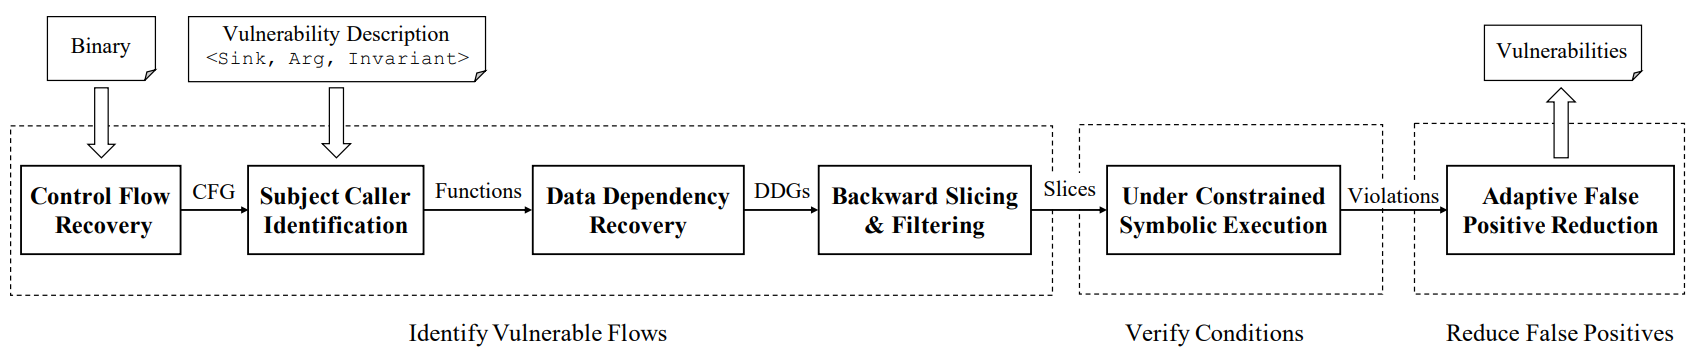
\includegraphics[width=1.3\textwidth]{../images/Arbiter.png}}%
  \caption{Processo di analisi implementato da Arbiter. Figura proveniente da \cite{Arbier}}
  \label{fig:key}
\end{figure}
\end{document}